% SSW 590 DevOps Assignment Template
% Developed by Darian Muresan, Ph.D., with OpenAI Codex and Anthropic Claude Code.
% AI agents: read devopsAIAgentGuide.tex before editing this template.
\documentclass[12pt]{cornell}

\usepackage[T1]{fontenc}
\usepackage{lmodern}
\usepackage{xspace}
\usepackage{xcolor}
\usepackage{graphicx}
\usepackage{fancyhdr}
\usepackage{amsmath,amssymb}
\usepackage{array}
\usepackage{booktabs}
\usepackage{longtable}
\usepackage{tabularx}
\usepackage{ltablex}
\keepXColumns
\usepackage{enumitem}
\usepackage{listings}
\usepackage{minted}
\usepackage{tcolorbox}
\usepackage{makeidx}
\usepackage{tikz}
% Symbols printed by the Node.js test runner in captured evidence
\DeclareUnicodeCharacter{2714}{\ensuremath{\checkmark}}
\DeclareUnicodeCharacter{2716}{\ensuremath{\times}}
\DeclareUnicodeCharacter{2139}{\textit{i}}
\usetikzlibrary{shapes.multipart,arrows.meta,positioning}
\usepackage[colorlinks=true,citecolor=blue,linkcolor=blue,urlcolor=blue]{hyperref}
\usepackage[acronym,toc]{glossaries}

\makeindex
\makeglossaries
\newacronym{ai}{AI}{artificial intelligence}
\newacronym{ci}{CI}{continuous integration}
\newacronym{cd}{CD}{continuous delivery or continuous deployment}
\newacronym{iac}{IaC}{infrastructure as code}
\newacronym{slo}{SLO}{service-level objective}
\newglossaryentry{automation}{name={automation},description={A repeatable, version-controlled procedure executed by software rather than undocumented manual steps}}
\newglossaryentry{container}{name={container},description={An isolated, runnable instance of a container image that packages an application with its dependencies}}
\newglossaryentry{containerimage}{name={container image},description={An immutable, layered template built from a Dockerfile from which containers are started}}
\newglossaryentry{deployment}{name={deployment},description={The controlled delivery of a versioned change to an environment}}
\newglossaryentry{evidence}{name={evidence},description={A retained record of an actual execution, observation, or review}}
\newglossaryentry{kanban}{name={Kanban board},description={A visual workflow board with columns such as To Do, In Progress, and Complete, used to make work and work-in-progress visible}}
\newglossaryentry{observability}{name={observability},description={The ability to infer system behavior from signals such as logs, metrics, traces, and health checks}}
\newglossaryentry{pipeline}{name={pipeline},description={An automated sequence that builds, tests, packages, and/or deploys a change}}
\newglossaryentry{rollback}{name={rollback},description={A controlled return to a known acceptable version or state after a failed or harmful change}}
\newglossaryentry{runbook}{name={runbook},description={A documented operational procedure for a repeatable task or incident response}}
\newglossaryentry{synonyms}{name={synonyms},description={Equivalent terms used in this assignment; record preferred terms to avoid ambiguity in instructions and evidence}}
\newacronym{aws}{AWS}{Amazon Web Services}
\newacronym{ec2}{EC2}{Amazon Elastic Compute Cloud}
\newacronym{ami}{AMI}{Amazon Machine Image}
\newacronym{uml}{UML}{Unified Modeling Language}
\newacronym{dora}{DORA}{DevOps Research and Assessment}
\newacronym{swot}{SWOT}{strengths, weaknesses, opportunities, and threats}
\newglossaryentry{securitygroup}{name={security group},description={A stateful virtual firewall attached to an AWS instance that lists the inbound and outbound traffic it allows}}
\newglossaryentry{userdata}{name={user data},description={A script supplied when an EC2 instance is launched that runs once as root at first boot}}
\newglossaryentry{texlive}{name={TeX Live},description={A cross-platform distribution of TeX, LaTeX, and their packages; Overleaf compiles projects with it}}


\definecolor{devopsBlue}{RGB}{31,78,121}
\definecolor{devopsGreen}{RGB}{46,125,50}
\definecolor{devopsRed}{RGB}{183,28,28}
\definecolor{devopsGray}{RGB}{90,90,90}
\definecolor{devopsLightBlue}{RGB}{232,240,247}

% Replace these values for each assignment.
\newcommand{\AssignmentTitle}{Cloud Docker Deployment and Project Proposal}
\newcommand{\AssignmentNumber}{4}
\newcommand{\DocumentVersion}{2.0}
\newcommand{\DocumentStatus}{Group 1 Submission}
\newcommand{\CourseNumber}{SSW 590}
\newcommand{\CourseName}{DevOps}
\newcommand{\Instructor}{David Darian Muresan, Ph.D.}
\newcommand{\StudentName}{Group 1: Brahmi Dalvi and Sakshi Deshpande}
\newcommand{\Organization}{Stevens Institute of Technology}
\newcommand{\DocumentDate}{October 6, 2026}
\newcommand{\DueDate}{[due date from Canvas]}
\newcommand{\VERSION}{Version \DocumentVersion}
% Public address of the AWS EC2 web server. Replace after running
% deploy/aws/launch-ec2.sh (see the AWS Docker Deployment chapter).
\newcommand{\WebsiteURL}{http://[EC2-PUBLIC-DNS]}
\newcommand{\RepoURL}{https://github.com/brahmi9811/ssw-590-group1}

\hypersetup{
  pdftitle={\CourseNumber\ --- Assignment \AssignmentNumber: \AssignmentTitle},
  pdfauthor={\StudentName},
  pdfcreator={Darian Muresan, Ph.D., with OpenAI Codex and Anthropic Claude Code},
  pdfsubject={Reusable DevOps course assignment template},
  pdfkeywords={DevOps, automation, delivery pipeline, infrastructure as code, evidence}
}

\newcolumntype{Y}{>{\raggedright\arraybackslash}X}
\newcolumntype{L}[1]{>{\raggedright\arraybackslash}p{#1}}
\setlength{\tabcolsep}{4pt}
\renewcommand{\arraystretch}{1.12}
\setlength{\LTpre}{6pt}
\setlength{\LTpost}{6pt}

% Stable IDs make activity, evidence, and artifact references durable.
\newcommand{\ArtifactLabel}[2]{\phantomsection\label{#1:#2}}
\newcommand{\ArtifactID}[2]{\texttt{#2}\ArtifactLabel{#1}{#2}\index{#1!#2}}
\newcommand{\ArtifactRef}[2]{\hyperref[#1:#2]{\texttt{#2}}}
\newcommand{\ActivityID}[1]{\ArtifactID{Activity}{#1}}
\newcommand{\ActivityRef}[1]{\ArtifactRef{Activity}{#1}}
\newcommand{\EvidenceID}[1]{\ArtifactID{Evidence}{#1}}
\newcommand{\EvidenceRef}[1]{\ArtifactRef{Evidence}{#1}}
\newcommand{\ChapterLabel}[1]{\label{Chapter:#1}}
\newcommand{\ChapterRef}[1]{\hyperref[Chapter:#1]{Chapter~\ref*{Chapter:#1}}}
\newcommand{\StatusPass}{\textbf{\footnotesize\textcolor{devopsGreen}{PASS}}}
\newcommand{\StatusPending}{\textbf{\footnotesize\textcolor{devopsGray}{PENDING}}}
\newcommand{\StatusFail}{\textbf{\footnotesize\textcolor{devopsRed}{FAIL}}}

\newtcolorbox{devopsNote}[1][]{
  colback=devopsLightBlue, colframe=devopsBlue, boxrule=0.6pt, arc=1mm, title=#1
}

\lstset{
  backgroundcolor=\color{white}, basicstyle=\ttfamily\footnotesize,
  breaklines=true, frame=single, keywordstyle=\color{blue},
  commentstyle=\color{devopsGreen}, numbers=left, numbersep=6pt,
  numberstyle=\tiny\color{devopsGray}, showstringspaces=false,
  stringstyle=\color{devopsRed}, tabsize=2
}
\setminted{fontsize=\footnotesize, breaklines, breakanywhere, frame=lines, framesep=2mm}

\setlength{\emergencystretch}{3em}
\changenormalspacing{\singlespacing}
\begin{document}
\pagenumbering{roman}
\singlespacing
\title{\CourseNumber\ --- \CourseName\\[0.5em]\large Assignment \AssignmentNumber: \AssignmentTitle\\[1.5em]\normalsize\VERSION\\\DocumentStatus}
\author{\StudentName\\\Organization}
\conferraldate{}{\DocumentDate}
\copyrightholder{\Organization}
\copyrightyear{2026}
\maketitle
\makecopyright

\cleardoublepage
\phantomsection
\chapter*{Template Attribution}
\ChapterLabel{TemplateAttribution}
\addcontentsline{toc}{chapter}{Template Attribution}
\markboth{Template Attribution}{Template Attribution}
\index{template attribution}
\index{Muresan, Darian}
This DevOps assignment template was developed by \textbf{Darian Muresan, Ph.D.},
in conjunction with \textbf{OpenAI Codex} and \textbf{Anthropic Claude Code}.

\clearpage
\begin{abstract}This group document records four SSW 590 activities completed by Group~1. We
deploy a Dockerized two-button website to a cloud virtual machine on Amazon Web
Services (AWS), which the group chose in place of a Digital Ocean Droplet;
refactor the website's button logic into class-based JavaScript and document
it with a UML class diagram; build a Docker container that compiles LaTeX with
TeX Live, the same distribution Overleaf uses; and propose the semester project,
a side-by-side DevSecOps comparison of two CI/CD tools delivering the same
containerized application to AWS. All code, deployment scripts, and evidence
live in the group repository so that every result can be reproduced.
\end{abstract}
\chapter*{Document History}
\addcontentsline{toc}{chapter}{Document History}
\index{document history}
\section*{How to Use This Chapter}
Add the newest approved change at the top. Retain every approved entry and
link each entry to the changed chapter, table, figure, or controlled artifact.
Author initials: BD = Brahmi Dalvi, SD = Sakshi Deshpande, CC = Claude Code
(AI assistant; see the AI Prompt Log), DDM = Darian Muresan, CDX = OpenAI Codex.

\begin{tabularx}{\linewidth}{L{3.1cm}L{2.2cm}YL{2.0cm}}
\caption{Document Update History\label{Table:DocumentHistory}}\\
\toprule \textbf{Date / Version} & \textbf{Author Initials} & \textbf{Change} & \textbf{Changed At}\\ \midrule
\endfirsthead
\multicolumn{4}{l}{\small\itshape Document Update History (continued)}\\
\toprule \textbf{Date / Version} & \textbf{Author Initials} & \textbf{Change} & \textbf{Changed At}\\ \midrule
\endhead \bottomrule \endlastfoot
October 7, 2026 / 2.1 & BD, CC & Executed the AWS EC2 deployment described in the AWS Docker Deployment chapter: launched instance \texttt{i-00ee7edd4a5352f05} (\texttt{t3.micro}, Amazon Linux 2023) with the \texttt{launch-ec2.sh} key pair and security group. The bootstrap script's anonymous \texttt{git clone} failed because the group repository is private; diagnosed from the real EC2 console output and fixed by adding a read-only GitHub deploy key and completing the clone, Docker build, and container run by hand over SSH. A browser could not open the resulting plain-HTTP site (silent HTTPS upgrade on \texttt{amazonaws.com} hosts hitting a closed port 443), diagnosed with \texttt{curl}/\texttt{Invoke-WebRequest}/\texttt{Test-NetConnection} from a working machine against a failing browser and phone; fixed by opening port 443 and adding an \texttt{nginx} TLS reverse proxy with a self-signed certificate, which itself needed a stray default \texttt{listen 80} server block removed from \texttt{nginx.conf}. Verified the live site over both HTTP and HTTPS, captured a real browser screenshot, and marked every row of the deployment checklist \StatusPass. Set the real \texttt{\string\WebsiteURL} and updated the Security Notes section to match. & \ChapterRef{AWSDockerDeployment}\\
October 6, 2026 / 2.0 & SD, CC & Created the Group~1 document in the group repository from the individual template. Added the AWS Docker Deployment chapter (AWS EC2 in place of a Digital Ocean Droplet, with Console and CLI steps in \texttt{minted}), the Class-Based Two-Button Website chapter with a UML class diagram and unit tests, the LaTeX Docker chapter (TeX Live container with real build output), and the Project Proposal chapter (TwinTrack: GitHub Actions vs.\ Jenkins, dashboard, modified SWOT charts). Switched the build to the LaTeX container and added AWS, EC2, UML, DORA, and SWOT glossary terms. & \ChapterRef{AWSDockerDeployment}, \ChapterRef{ClassBasedWebsite}, \ChapterRef{LatexDocker}, \ChapterRef{ProjectProposal}, \ChapterRef{DocumentGuide}\\
September 2, 2026 / 1.0--1.3 & DDM, CDX & Created the reusable SSW 590 DevOps assignment template, the one-file-per-chapter convention, and the authoring guide. & \ChapterRef{DocumentGuide}, \ChapterRef{AIAgentGuide}\\
\textit{[date / version]} & \textit{[initials]} & \textit{[approved change and rationale]} & \textit{[link]}\\
\end{tabularx}

\contentspage
\tablelistpage
\figurelistpage


\setcounter{page}{1}
\pagenumbering{arabic}
\pagestyle{fancy}
\fancyhf{}
\renewcommand{\chaptermark}[1]{\markboth{#1}{}}
\lhead{\small Assignment \AssignmentNumber}
\chead{\small\nouppercase{\leftmark}}
\rhead{\small\thepage}
\lfoot{\small\CourseNumber}
\cfoot{\small\copyright\ \Organization}
\rfoot{\small\VERSION}
\renewcommand{\headrulewidth}{0.4pt}
\renewcommand{\footrulewidth}{0.4pt}

\chapter{Introduction}
\ChapterLabel{Introduction}
\index{introduction}
\index{DevOps}

\section{Purpose}
This is the shared Group~1 document for SSW~590. It collects the group's
deployment work, supporting containers, and project proposal in one place, and
it is maintained in the group repository alongside the code it describes.

\section{Team and Repository}
\begin{tabularx}{\linewidth}{L{3.6cm}Y}
\toprule \textbf{Item} & \textbf{Value}\\ \midrule
Group & Group 1\\
Members & Brahmi Dalvi (BD), Sakshi Deshpande (SD)\\
Repository & \url{\RepoURL}\\
Cloud provider & \gls{aws} (disclosed group substitution for the assignment's Digital Ocean Droplet; see \ChapterRef{AWSDockerDeployment})\\
Due date & \DueDate\\ \bottomrule
\end{tabularx}

\section{Repository Layout}
\begin{minted}{text}
ssw-590-group1/
  website/color-buttons-app/   two-button site (class-based JS) + Dockerfile
  deploy/aws/                  EC2 launch, user-data, redeploy, teardown scripts
  latex-docker/                TeX Live container that compiles LaTeX
  evidence/                    captured command output from real runs
  docs/                        UML source (Mermaid) and other notes
  report/                      this LaTeX document
\end{minted}

\section{Chapter Map}
\begin{tabularx}{\linewidth}{L{5.2cm}Y}
\toprule \textbf{Assignment item} & \textbf{Where it is answered}\\ \midrule
1--2. Cloud Docker deployment & \ChapterRef{AWSDockerDeployment}\\
3. Class-based JavaScript and UML & \ChapterRef{ClassBasedWebsite}\\
4. LaTeX Docker & \ChapterRef{LatexDocker}\\
5--6. Project proposal and rubric & \ChapterRef{ProjectProposal}\\
7. Document history & Document History (front matter)\\ \bottomrule
\end{tabularx}

\section{Use of AI}
AI assistance is recorded in \ChapterRef{AIPromptLog}. Members reviewed every
command and result before including it.

\chapter{AWS Docker Deployment}
\ChapterLabel{AWSDockerDeployment}
\index{AWS}
\index{EC2}
\index{Docker!cloud deployment}

\section{Overview}
\begin{devopsNote}[Deviation from the assignment, disclosed]
This assignment's instructions ask for a \textbf{Digital Ocean Droplet}
running Docker. Group~1 deployed to an \textbf{AWS EC2 instance} instead,
performing the exact same role: one cloud virtual machine running Docker and
serving the website. This substitution is a group choice, not something the
assignment itself offered for this item; it is made because the semester
project (\ChapterRef{ProjectProposal}) is built on AWS, and standing up the
account, IAM users, budget alert, and security-group model here means that
work is reused rather than duplicated on a second cloud provider the group
would not otherwise use. Table~\ref{Table:DOtoAWS} maps every Digital Ocean
concept the assignment describes onto its AWS equivalent, so the deployment
can be read and graded as a direct substitute. If a literal Digital Ocean
Droplet is required, the group will redeploy there using \texttt{doctl} in
place of the AWS CLI; the Docker image and application are unchanged either
way.
\end{devopsNote}
The cloud server is an \gls{ec2} instance, which plays the role of a Droplet.
It runs the two-button website from \ChapterRef{ClassBasedWebsite} in a
Docker container and serves it on port~80.

\begin{devopsNote}[Live website]
\textbf{Website:} \texttt{\WebsiteURL}\\
\textbf{Health check:} \texttt{\WebsiteURL/health}\\
\textbf{Source:} \url{\RepoURL}\\[3pt]
\small The address is set by the \texttt{\string\WebsiteURL} macro in
\texttt{devopsAssignment.tex}. Replace the placeholder with the public DNS name
printed by \texttt{launch-ec2.sh} (Section~\ref{Section:AWSCLI}).
\end{devopsNote}

\section{Digital Ocean to AWS Mapping}
\begin{tabularx}{\linewidth}{L{3.6cm}L{4.4cm}Y}
\caption{Digital Ocean Concepts and Their AWS Equivalents\label{Table:DOtoAWS}}\\
\toprule \textbf{Digital Ocean} & \textbf{AWS} & \textbf{Used here}\\ \midrule
\endfirsthead
\toprule \textbf{Digital Ocean} & \textbf{AWS} & \textbf{Used here}\\ \midrule
\endhead \bottomrule \endlastfoot
Droplet & \gls{ec2} instance & \texttt{t3.micro}, Free Tier eligible\\
Droplet image (Ubuntu) & \gls{ami} & Amazon Linux 2023\\
Cloud Firewall & \gls{securitygroup} & HTTP 80 and HTTPS 443 open; SSH 22 from one IP\\
SSH key & EC2 key pair & \texttt{ssw590-group1-key}\\
Cloud-init user data & EC2 \gls{userdata} & \texttt{deploy/aws/ec2-user-data.sh}\\
\texttt{doctl} CLI & AWS CLI v2 & \texttt{deploy/aws/launch-ec2.sh}\\
Docker 1-Click Droplet & Docker installed by \texttt{dnf} & Docker from the AL2023 repository\\
\end{tabularx}

\section{Prerequisites and Account Security}
\begin{enumerate}
\item Create an AWS account and enable multi-factor authentication on the root
user. Do not use the root user for daily work.
\item In IAM, create a user for each member with console access and the
\texttt{AmazonEC2FullAccess} policy (or a narrower custom policy), and create an
access key for CLI use. Keys are stored only in \texttt{\textasciitilde/.aws/credentials}
on the member's machine and are never committed.
\item In Billing, create a monthly budget (for example \$5) with an e-mail
alert so a forgotten instance is noticed quickly.
\item Install and configure the AWS CLI v2:
\end{enumerate}
\begin{minted}{bash}
brew install awscli                # macOS; see AWS docs for Windows/Linux
aws configure                      # access key, secret, region us-east-1, output json
aws sts get-caller-identity        # confirms the CLI is signed in as the IAM user
\end{minted}

\section{Deployment Steps}
Two equivalent paths are documented: the AWS Console (closest to creating a
Droplet in the Digital Ocean web UI) and a scripted CLI path that the group uses
for repeatable deployments. Both run the same \gls{userdata} script.

\subsection{The Bootstrap Script}
\label{Section:Bootstrap}
At first boot the instance runs this script as root. It installs Docker and Git,
clones the group repository, builds the image, and starts the container with a
restart policy so the site comes back after a reboot. Port~80 on the host is
mapped to port~3000 inside the container.
\inputminted{bash}{../deploy/aws/ec2-user-data.sh}

\subsection{Private Repository and the Deploy Key}
\label{Section:DeployKey}
\begin{devopsNote}[What actually happened on this deployment]
The group repository is \textbf{private}. The bootstrap script in
Section~\ref{Section:Bootstrap} clones it anonymously over HTTPS, which works
only for a public repository. On the real run, cloud-init's \gls{userdata}
step failed with \texttt{fatal: could not read Username for
`https://github.com': No such device or address}, so the container never
started automatically. This was diagnosed from the instance's console output
(\texttt{aws ec2 get-console-output}) rather than guessed.

The fix was to generate an \texttt{ed25519} key pair on the instance, add its
\emph{public} half as a read-only \textbf{deploy key} on the GitHub repository
(Settings $\rightarrow$ Deploy keys), and then run the same clone, build, and
run commands shown in Section~\ref{Section:ManualCommands} by hand over SSH,
using \texttt{git@github.com:\dots} instead of the HTTPS URL. The private key
never leaves the instance; the deploy key is read-only and scoped to this one
repository. A future improvement would be to bake the deploy key into the AMI
or pass it through \gls{userdata} (e.g.\ via AWS Secrets Manager) so first
boot succeeds without a manual step; that is not yet done.
\end{devopsNote}

\subsection{Path A: AWS Console}
\begin{enumerate}
\item Open \textbf{EC2 $\rightarrow$ Launch instance}. Name it
\texttt{ssw590-group1-web}.
\item Choose the \textbf{Amazon Linux 2023} \gls{ami} (64-bit x86) and instance
type \textbf{t3.micro}.
\item Under \textbf{Key pair}, create \texttt{ssw590-group1-key} (RSA,
\texttt{.pem}) and save the downloaded file to \texttt{\textasciitilde/.ssh/}.
\item Under \textbf{Network settings}, create a security group that allows
\textbf{SSH} from \emph{My IP} and \textbf{HTTP} from \emph{Anywhere}.
\item Expand \textbf{Advanced details}. In the \textbf{User data} box, paste
the contents of \path{deploy/aws/ec2-user-data.sh}.
\item Click \textbf{Launch instance}, wait for \emph{2/2 status checks passed},
and copy the \textbf{Public IPv4 DNS} from the instance page.
\end{enumerate}

\subsection{Path B: AWS CLI}
\label{Section:AWSCLI}
The launch script creates the key pair and security group if they do not exist,
looks up the latest Amazon Linux 2023 \gls{ami} from AWS's public SSM parameter,
launches the instance with the bootstrap script, and prints the website address.
\inputminted{bash}{../deploy/aws/launch-ec2.sh}
It is run from the repository root:
\begin{minted}{bash}
git clone https://github.com/brahmi9811/ssw-590-group1.git
cd ssw-590-group1
./deploy/aws/launch-ec2.sh
\end{minted}

\subsection{Manual Commands on the Instance}
\label{Section:ManualCommands}
For transparency, these are the same steps the bootstrap script automates,
typed by hand after connecting over SSH. They are also the steps to follow if
the user data is omitted.
\begin{minted}{bash}
chmod 400 ~/.ssh/ssw590-group1-key.pem
ssh -i ~/.ssh/ssw590-group1-key.pem ec2-user@<EC2-PUBLIC-DNS>

# on the instance
sudo dnf update -y
sudo dnf install -y docker git
sudo systemctl enable --now docker
sudo usermod -aG docker ec2-user && newgrp docker
docker --version

git clone https://github.com/brahmi9811/ssw-590-group1.git
cd ssw-590-group1/website/color-buttons-app
docker build -t color-buttons-app:2.0 .
docker run -d --name color-buttons-app --restart unless-stopped \
  -p 80:3000 color-buttons-app:2.0
docker ps
\end{minted}

\section{Verification}
\subsection{Pre-deployment Check on a Workstation}
Before deploying, the exact image that the instance builds was built and run on
a group member's workstation (Docker 29.4.2, Apple silicon), published on host
port~8081. The output below is from that real run.
\inputminted{console}{../evidence/local-build-run.txt}
\inputminted{console}{../evidence/local-checks.txt}
The page was then opened in a browser; clicking \emph{Red} and then \emph{Blue}
changed the page background to red and then blue, served by the class-based
code in \ChapterRef{ClassBasedWebsite}.

\subsection{Cloud Verification}
After launch, the following commands confirm the deployment from any machine.
Paste their output into \path{evidence/aws-checks.txt} and save a browser
screenshot as \path{evidence/aws-website.png}.
\begin{minted}{bash}
curl -s http://<EC2-PUBLIC-DNS>/health        # {"status":"ok",...}
curl -sI http://<EC2-PUBLIC-DNS>/ | head -1   # HTTP/1.1 200 OK
ssh -i ~/.ssh/ssw590-group1-key.pem ec2-user@<EC2-PUBLIC-DNS> \
  'docker ps --format "{{.Names}} {{.Status}} {{.Ports}}"'
\end{minted}
\inputminted{console}{../evidence/aws-checks.txt}

\begin{devopsNote}[A browser-only problem, and why port 443 is also open]
\texttt{curl} reached the site over plain HTTP the whole time, but a browser
pointed at the same \texttt{http://} address showed
\texttt{ERR\_CONNECTION\_TIMED\_OUT}. The cause was not the server: current
Chrome and mobile browsers silently upgrade \texttt{http://} requests on
\texttt{amazonaws.com} hosts to \texttt{https://} (an HSTS/HTTPS-first
behavior that is hard-coded for many cloud domains and is not something a
per-site browser setting can turn off), so the browser was actually trying
port~443, which the security group did not yet open. The fix was to open
port~443 (Table~\ref{Table:DOtoAWS}'s security group) and put
\texttt{nginx} in front of the container as a TLS-terminating reverse proxy
on port~443, forwarding to the existing app on port~80. The connection now
succeeds for any browser on any network. Figure~\ref{Figure:AWSWebsite}
shows the deployed site in a browser, including the two-button click
behavior working against the live cloud instance.
\end{devopsNote}

\begin{figure}[htbp]
\centering
\fbox{
\includegraphics[width=0.7\linewidth]{../evidence/aws-website.png}}
\caption{The deployed site at the public EC2 address, on load.}
\label{Figure:AWSWebsite}
\end{figure}

\begin{figure}[htbp]
\centering
\fbox{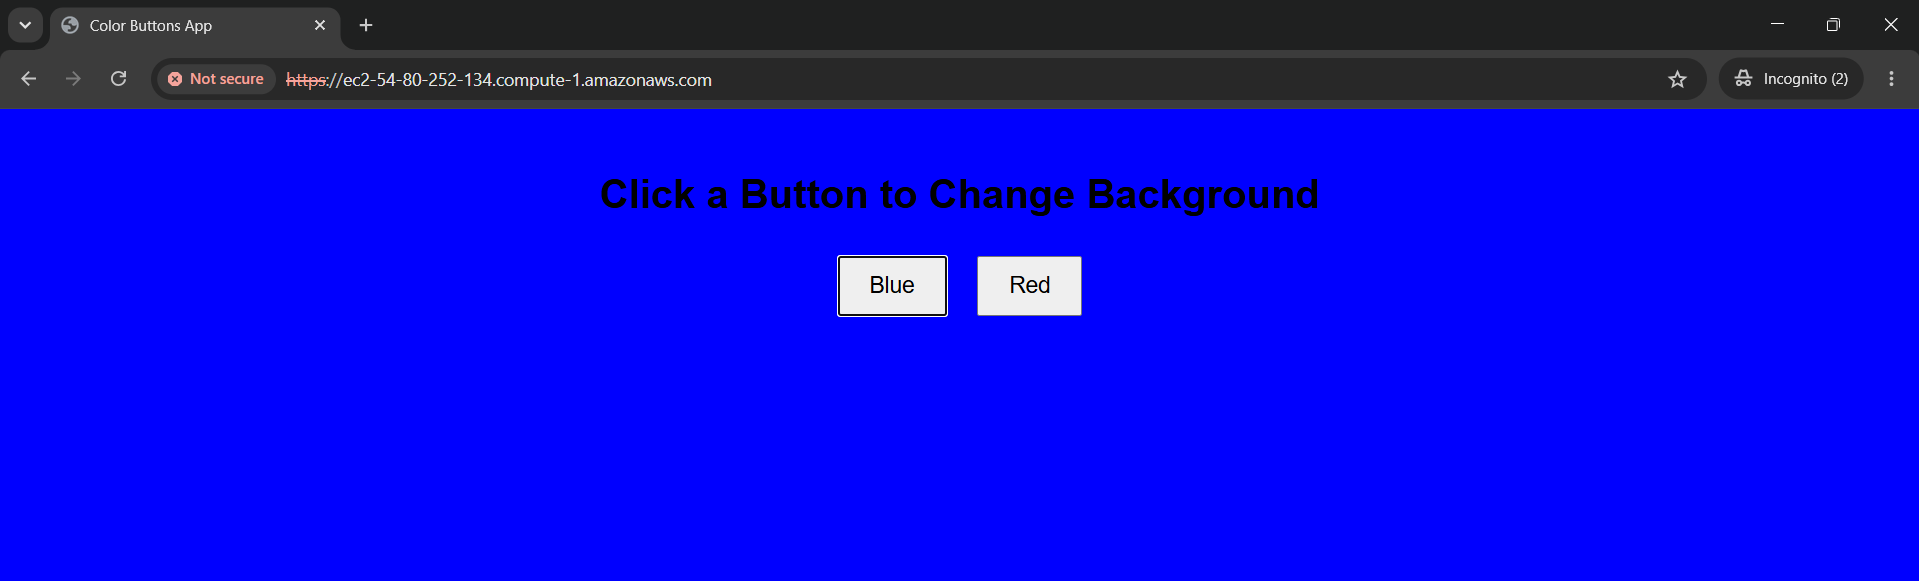
\includegraphics[width=0.7\linewidth]{../evidence/aws-website-blue.png}}
\caption{The same deployment after clicking \emph{Blue}.}
\label{Figure:AWSWebsiteBlue}
\end{figure}

\begin{figure}[htbp]
\centering
\fbox{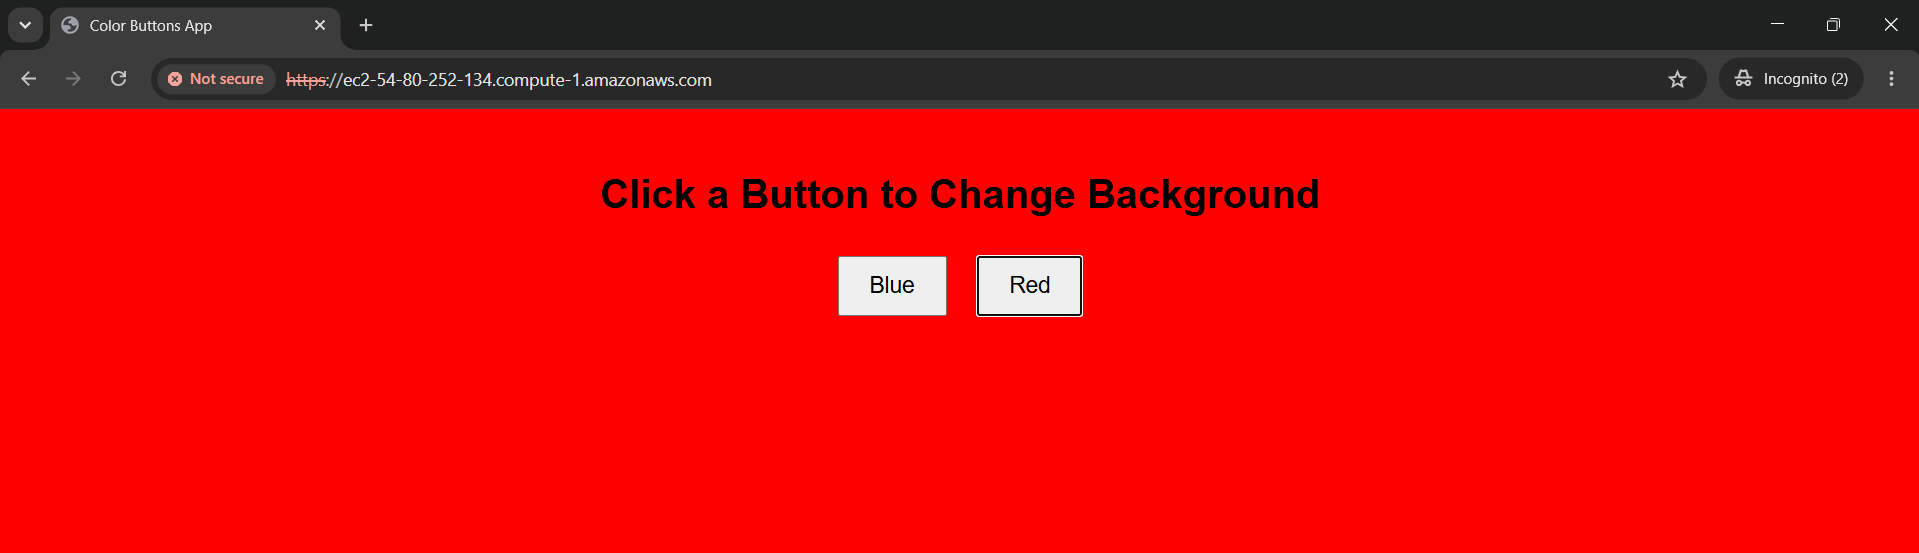
\includegraphics[width=0.7\linewidth]{../evidence/aws-website-red.png}}
\caption{The same deployment after clicking \emph{Red}. Together with
Figures~\ref{Figure:AWSWebsite} and~\ref{Figure:AWSWebsiteBlue}, this
confirms the class-based code from \ChapterRef{ClassBasedWebsite} runs
correctly on the real cloud deployment, not just locally.}
\label{Figure:AWSWebsiteRed}
\end{figure}

\begin{tabularx}{\linewidth}{L{5.2cm}L{2.2cm}Y}
\caption{Deployment Checklist\label{Table:AWSChecklist}}\\
\toprule \textbf{Check} & \textbf{Status} & \textbf{Evidence}\\ \midrule
\endfirsthead
\toprule \textbf{Check} & \textbf{Status} & \textbf{Evidence}\\ \midrule
\endhead \bottomrule \endlastfoot
Image builds and runs locally & \StatusPass & \texttt{evidence/local-build-run.txt}\\
\texttt{/health} and JS module served & \StatusPass & \texttt{evidence/local-checks.txt}\\
Buttons work in a browser & \StatusPass & Manual browser check (red, then blue)\\
EC2 instance launched & \StatusPass & \texttt{i-00ee7edd4a5352f05}, public DNS \texttt{ec2-54-80-252-134.compute-1.amazonaws.com}\\
Public URL returns HTTP 200 & \StatusPass & \texttt{evidence/aws-checks.txt}\\
Screenshot of public site & \StatusPass & \texttt{evidence/aws-website.png} (Figure~\ref{Figure:AWSWebsite})\\
\end{tabularx}

\section{Updating the Deployment}
After a change is merged to \texttt{main}, a member connects over SSH and runs
the redeploy script, which pulls the commit, rebuilds the image, and replaces
the container:
\inputminted{bash}{../deploy/aws/redeploy.sh}

\section{Security Notes}
\begin{itemize}
\item SSH is open only to the launching member's public IP. HTTP (80) and
HTTPS (443) are open to the internet; HTTPS was added, after deployment, for
the reason explained in Section~\ref{Section:ManualCommands}. The container
itself listens on 3000, which is not exposed directly.
\item No credentials are stored in the repository. The EC2 key pair's private
key and the IAM access key remain on members' machines. The repository itself
is private; the EC2 instance's own access to it is a read-only GitHub deploy
key (Section~\ref{Section:DeployKey}) that was added specifically for this
instance and grants no write access and no access to any other repository.
\item The site is served over HTTPS using \texttt{nginx} with a
\textbf{self-signed} certificate (Section~\ref{Section:DeployKey}
devopsNote), so browsers show a certificate warning that a user must click
through. A production setup would replace this with a certificate from a
real certificate authority (e.g.\ Let's Encrypt via \texttt{certbot}, or an
Application Load Balancer with an ACM certificate), which requires owning a
domain name the group did not acquire for this exercise.
\end{itemize}

\section{Cost and Teardown}
A \texttt{t3.micro} instance is Free Tier eligible for new accounts; outside
the Free Tier it costs roughly one US cent per hour plus storage, and AWS also
charges for public IPv4 addresses. When the site is no longer needed for
grading, terminate it:
\inputminted{bash}{../deploy/aws/teardown-ec2.sh}

\chapter{Class-Based Two-Button Website}
\ChapterLabel{ClassBasedWebsite}
\index{JavaScript!classes}
\index{UML}

\section{Overview}
The original website attached two anonymous arrow functions directly to the
Blue and Red buttons. Each function repeated the same logic with a different
color. This chapter replaces those inline handlers with three ES2015 classes in
\texttt{public/js/colorButtons.js}, loaded by the page as a JavaScript module.
The visible behavior is unchanged.

\section{Original Design}
\begin{minted}{html}
<script>
  document.getElementById("blueBtn").addEventListener("click", () => {
    document.body.style.backgroundColor = "blue";
  });

  document.getElementById("redBtn").addEventListener("click", () => {
    document.body.style.backgroundColor = "red";
  });
</script>
\end{minted}

\section{Class-Based Design}
\begin{itemize}
\item \textbf{\texttt{BackgroundChanger}} owns the element whose background
changes (the page body) and is the only class that touches its style.
\item \textbf{\texttt{ColorButton}} binds one button element to one color and
delegates the change to a \texttt{BackgroundChanger}.
\item \textbf{\texttt{ColorButtonApp}} holds the button configuration,
creates
one shared \texttt{BackgroundChanger} and one \texttt{ColorButton} per entry,
and binds them. Adding a third color is a one-line change to
\texttt{BUTTONS}.
\end{itemize}

\subsection{UML Class Diagram}
Figure~\ref{Figure:ColorButtonsUML} shows the updated design. A filled diamond
marks composition: the application creates and owns its buttons and its
background changer. The plain arrow is a directed association: each button
holds a reference to the shared changer. An underlined attribute is static;
\texttt{-} marks a field that is private by convention and \texttt{+} a public
method. The same diagram is kept as Mermaid
source in \texttt{docs/uml-class-diagram.md}, which GitHub renders directly.

\begin{figure}[htbp]
\centering
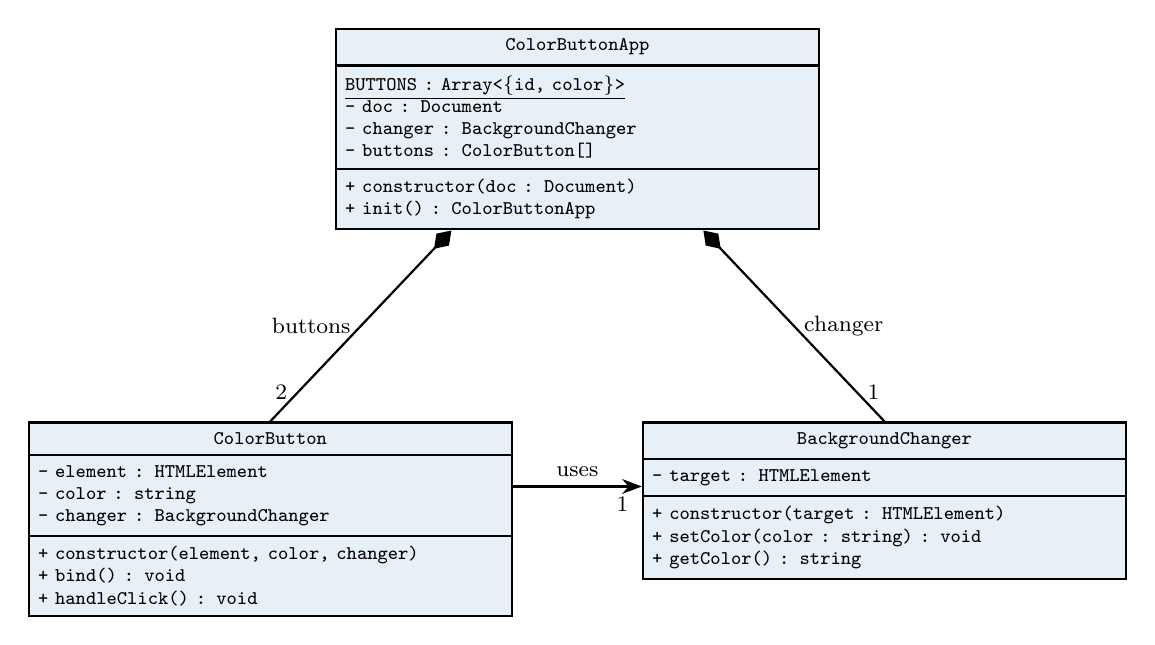
\begin{tikzpicture}[
  umlclass/.style={rectangle split, rectangle split parts=3, draw, thick,
    fill=devopsLightBlue, text width=5.9cm, font=\ttfamily\scriptsize},
  comp/.style={{Diamond[length=3.2mm,width=2.2mm]}-, thick},
  lbl/.style={font=\footnotesize}]
\node[umlclass, anchor=north] (app) at (0,0) {\hfill\textbf{ColorButtonApp}\hfill\null
  \nodepart{second}
  \underline{BUTTONS : Array<\{id, color\}>}\\
  - doc : Document\\
  - changer : BackgroundChanger\\
  - buttons : ColorButton[]
  \nodepart{third}
  + constructor(doc : Document)\\
  + init() : ColorButtonApp};
\node[umlclass, anchor=north] (btn) at (-3.9,-5.0) {\hfill\textbf{ColorButton}\hfill\null
  \nodepart{second}
  - element : HTMLElement\\
  - color : string\\
  - changer : BackgroundChanger
  \nodepart{third}
  + constructor(element, color, changer)\\
  + bind() : void\\
  + handleClick() : void};
\node[umlclass, anchor=north] (chg) at (3.9,-5.0) {\hfill\textbf{BackgroundChanger}\hfill\null
  \nodepart{second}
  - target : HTMLElement
  \nodepart{third}
  + constructor(target : HTMLElement)\\
  + setColor(color : string) : void\\
  + getColor() : string};
\draw[comp] ([xshift=-1.6cm]app.south) -- (btn.north)
  node[lbl, pos=0.85, left] {2} node[lbl, midway, left] {buttons};
\draw[comp] ([xshift=1.6cm]app.south) -- (chg.north)
  node[lbl, pos=0.85, right] {1} node[lbl, midway, right] {changer};
\draw[-{Stealth[length=2.5mm]}, thick] ([yshift=-4mm]btn.text split east) -- ([yshift=-4mm]btn.text split east -| chg.west)
  node[lbl, midway, above] {uses} node[lbl, pos=0.85, below] {1};
\end{tikzpicture}
\caption{UML class diagram of the class-based two-button website.}
\label{Figure:ColorButtonsUML}
\end{figure}

\section{Implementation}
\noindent\textbf{public/js/colorButtons.js} --- the three classes, exported as
an ES module so the browser and the unit tests load the same file:
\inputminted{javascript}{../website/color-buttons-app/public/js/colorButtons.js}

\medskip\noindent\textbf{public/index.html} --- the page now loads the module
and creates the application in two lines:
\inputminted{html}{../website/color-buttons-app/public/index.html}

\medskip\noindent\textbf{server.js} --- unchanged except for a
\texttt{/health} endpoint used by the deployment checks in
\ChapterRef{AWSDockerDeployment}:
\inputminted{javascript}{../website/color-buttons-app/server.js}

\medskip\noindent\textbf{Dockerfile} --- unchanged from the local Docker
exercise. A new \texttt{.dockerignore} keeps \texttt{node\_modules} and the
tests out of the image.
\inputminted{docker}{../website/color-buttons-app/Dockerfile}

\section{Testing}
Because the classes receive the document and elements through their
constructors rather than reading globals, they can be tested in Node.js with
small stand-in objects, without a browser. The tests use Node's built-in
\texttt{node:test} runner, so no extra dependency is needed.
\inputminted{javascript}{../website/color-buttons-app/test/colorButtons.test.js}
Result of \texttt{npm test}:
\inputminted{console}{../evidence/website-unit-tests.txt}
The module was also loaded in a real browser from the running container, where
clicking \emph{Red} then \emph{Blue} set the body background to
\texttt{red} and then \texttt{blue}.

\chapter{LaTeX Docker}
\ChapterLabel{LatexDocker}
\index{LaTeX!Docker}
\index{TeX Live}
\index{Overleaf}

\section{Overview}
Overleaf compiles every project with \gls{texlive}, run inside containers on
its servers. This chapter reproduces that setup locally: a Docker image built on
the official \texttt{texlive/texlive} image compiles a simple LaTeX document
from a folder on the host. The same container builds this group document, so
every member gets an identical toolchain without installing MacTeX or MiKTeX,
and the build can later run unchanged in a CI pipeline.

\section{How It Works}
\begin{enumerate}
\item The image contains a full TeX Live installation plus \texttt{latexmk},
which reruns \texttt{pdflatex}, BibTeX, and index tools until cross-references
settle.
\item At run time the current host folder is bind-mounted at
\texttt{/workdir}, so the container reads the \texttt{.tex} source and writes
the PDF back to the host.
\item The container is started with \texttt{--rm}, so it is deleted after each
compile. Only the image persists.
\end{enumerate}

\section{Project Files}
\begin{minted}{text}
latex-docker/
  Dockerfile    image definition
  hello.tex     simple test document
  build.sh      builds the image and compiles a .tex file
  .gitignore    keeps auxiliary files out of Git
\end{minted}

\noindent\textbf{Dockerfile} --- \texttt{ENTRYPOINT} fixes the compiler and
flags, while \texttt{CMD} supplies a default file name that can be overridden on
the \texttt{docker run} line. \texttt{-shell-escape} is required by
\texttt{minted}; it lets LaTeX call the Pygments highlighter, so it should only
be used on trusted documents.
\inputminted{docker}{../latex-docker/Dockerfile}

\medskip\noindent\textbf{hello.tex} --- a small document that exercises text,
math, and a \texttt{minted} code block:
\inputminted{latex}{../latex-docker/hello.tex}

\medskip\noindent\textbf{build.sh} --- one command to build and compile:
\inputminted{bash}{../latex-docker/build.sh}

\section{Commands Run}
\subsection{Build the Image}
The base image is large (about 2.7\,GB compressed) because it contains the
complete TeX Live distribution, the same scheme Overleaf offers. It is pulled
once and then cached.
\begin{minted}{bash}
cd latex-docker
docker pull texlive/texlive:latest
docker build -t latex-builder .
\end{minted}
\inputminted{console}{../evidence/latex-docker-build.txt}

\subsection{Compile the Document}
\begin{minted}{bash}
docker run --rm -v "$PWD":/workdir latex-builder hello.tex
\end{minted}
The output below is abridged to \texttt{latexmk}'s run summary; the TeX Live
2026 \texttt{pdflatex} ran three times before reporting that the PDF was up to
date.
\inputminted{console}{../evidence/latex-docker-run.txt}
Figure~\ref{Figure:LatexDockerOutput} shows the resulting PDF.

\begin{figure}[htbp]
\centering
\setlength{\fboxsep}{0pt}\fbox{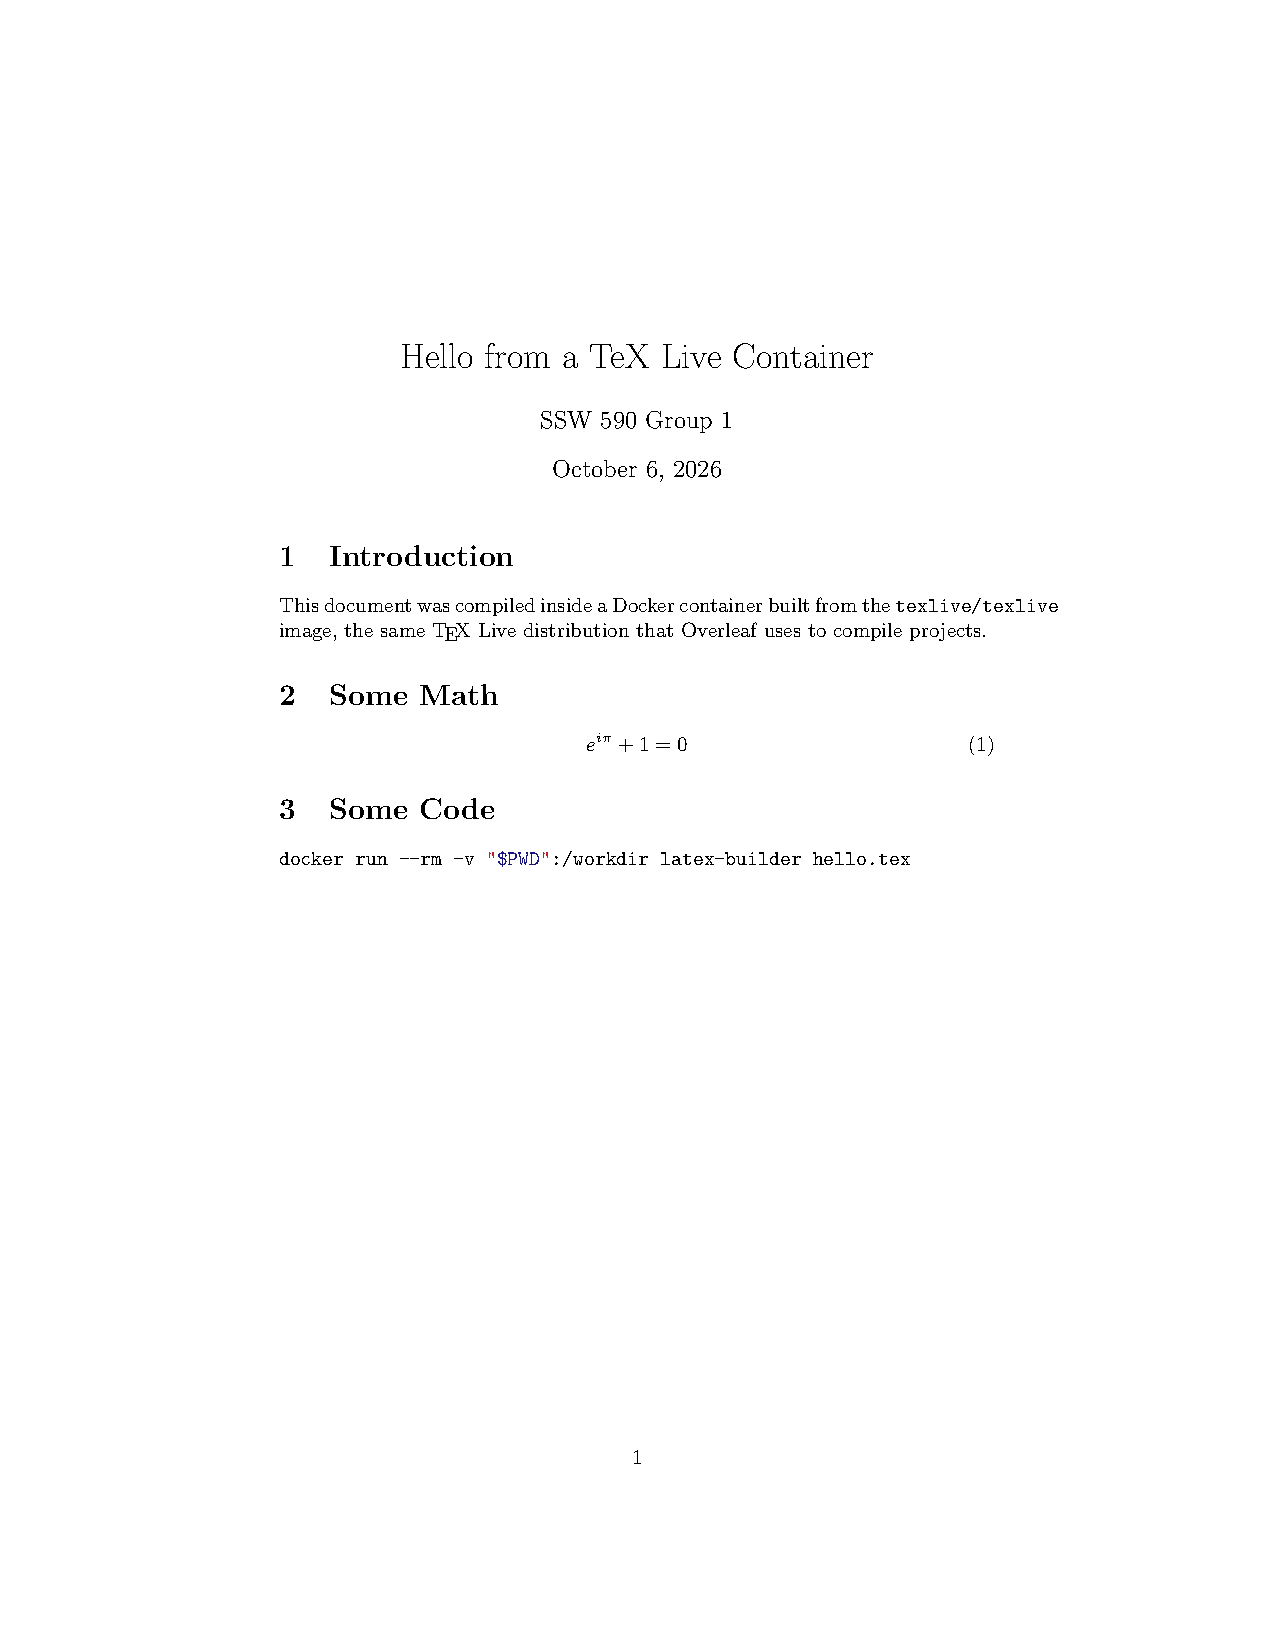
\includegraphics[width=0.75\linewidth,trim=90 420 90 90,clip]{../evidence/latex-docker-hello.pdf}}
\caption{Top of \texttt{hello.pdf} compiled by the \texttt{latex-builder} container.}
\label{Figure:LatexDockerOutput}
\end{figure}

\subsection{Compile This Group Document}
The same image builds this report. From the repository root, the whole
repository is mounted so the report can include source files from
\texttt{website/}, \texttt{deploy/}, and \texttt{evidence/}:
\begin{minted}{bash}
docker run --rm -v "$PWD":/workdir -w /workdir/report \
  latex-builder devopsAssignment.tex
\end{minted}

\section{Comparison with Overleaf}
\begin{tabularx}{\linewidth}{L{3.0cm}YY}
\caption{Overleaf Compared with the LaTeX Container\label{Table:OverleafVsDocker}}\\
\toprule \textbf{Aspect} & \textbf{Overleaf} & \textbf{LaTeX Docker}\\ \midrule
\endfirsthead
\toprule \textbf{Aspect} & \textbf{Overleaf} & \textbf{LaTeX Docker}\\ \midrule
\endhead \bottomrule \endlastfoot
Engine & TeX Live in server-side containers & TeX Live in a local container\\
Collaboration & Real-time editing and comments & Git branches and pull requests\\
Version control & Built-in history; Git sync on paid plans & Native Git in the group repo\\
Compile limits & Timeout on free plan & Limited only by the machine\\
Offline use & No & Yes, once the image is pulled\\
Automation & Manual recompile & Scriptable; reusable in CI (\ChapterRef{ProjectProposal})\\
\end{tabularx}

\section{Troubleshooting}
\begin{itemize}
\item \textbf{Apple silicon.} \texttt{texlive/texlive} publishes
\texttt{arm64} images, so it runs natively on Apple silicon Macs without
emulation.
\item \textbf{File not found.} The \texttt{.tex} file must be inside the
mounted folder; paths are resolved relative to \texttt{/workdir}.
\item \textbf{Glossaries.} \texttt{latexmk} does not run
\texttt{makeglossaries} by default; \texttt{report/latexmkrc} adds that rule
for this document.
\end{itemize}

\chapter{Project Proposal}
\ChapterLabel{ProjectProposal}
\index{project proposal}
\index{DevSecOps}
\index{SWOT}

\section{Title}
\begin{center}
\large\textbf{TwinTrack: A Side-by-Side DevSecOps Comparison of GitHub Actions
and Jenkins Delivering a Containerized Task Tracker to AWS}
\end{center}

\section{Project Description}
Group~1 will build one small but complete web application, \emph{TwinTrack},
a team task tracker, and deliver it to \gls{aws} through \textbf{two parallel
DevSecOps pipelines} built with comparable tools: \textbf{GitHub Actions}
(hosted, YAML-defined) and \textbf{Jenkins} (self-hosted, Groovy
\texttt{Jenkinsfile}). Both pipelines start from the same commit in the same
GitHub repository, run the same tests and security scans, build the same Docker
image, and deploy it to identical AWS environments (``blue'' for GitHub Actions,
``green'' for Jenkins). Because the application, tests, and target are held
constant, differences in speed, reliability, security coverage, cost, and
operator effort can be attributed to the pipeline tool itself.

An operations dashboard will collect metrics from both pipelines and both
running environments, and the group will finish with a modified \gls{swot}
chart for each tool and a recommendation for which tool suits which kind of
team.

\subsection{The Application}
TwinTrack is deliberately simple so the effort goes into DevOps rather than
features:
\begin{itemize}
\item A REST API (Node.js and Express, the stack from the two-button site) to
create, list, update, and close tasks, with a \texttt{/health} endpoint and a
Prometheus \texttt{/metrics} endpoint.
\item A small browser front end written with class-based JavaScript, following
the design in \ChapterRef{ClassBasedWebsite}.
\item A PostgreSQL database for tasks and users.
\end{itemize}

\subsection{Sample Tasks}
\begin{tabularx}{\linewidth}{L{1.0cm}YL{3.0cm}}
\caption{Sample Project Tasks\label{Table:ProposalTasks}}\\
\toprule \textbf{ID} & \textbf{Task} & \textbf{Area}\\ \midrule
\endfirsthead
\toprule \textbf{ID} & \textbf{Task} & \textbf{Area}\\ \midrule
\endhead \bottomrule \endlastfoot
T1 & Set up the GitHub repository, branch protection on \texttt{main}, pull-request template, and GitHub Projects Kanban board & Source control\\
T2 & Build the TwinTrack API and front end with Docker Compose for local development (app + PostgreSQL) & Development\\
T3 & Write unit, API, and end-to-end tests; enforce a coverage threshold & Testing\\
T4 & Provision two identical AWS environments (blue and green) with Terraform & Infrastructure as code\\
T5 & Write the GitHub Actions workflow: lint, test, scan, build, push to Amazon ECR, deploy to blue & CI/CD tool 1\\
T6 & Run Jenkins in Docker on EC2 and write an equivalent \texttt{Jenkinsfile} that deploys to green & CI/CD tool 2\\
T7 & Add security gates to both pipelines: secret scanning, dependency audit, container image scanning, and a DAST baseline scan & Security\\
T8 & Build the operations dashboard in Grafana (pipeline and runtime metrics) and compare with Amazon CloudWatch & Monitoring\\
T9 & Run the planted-fault experiment (Section~\ref{Section:Unique}) against both pipelines & Experiment\\
T10 & Write SWOT charts, comparison tables, and the final report; build the report with the LaTeX container from \ChapterRef{LatexDocker} & Documentation\\
\end{tabularx}

\section{DevSecOps Tools}
At this stage the list is intentionally broad; tools may be swapped as the
group learns more. Pairs marked ``vs.'' are candidates for head-to-head
comparison.

\begin{tabularx}{\linewidth}{L{2.8cm}YL{3.0cm}}
\caption{Planned DevSecOps Tool Chain\label{Table:ProposalTools}}\\
\toprule \textbf{Category} & \textbf{Tool(s)} & \textbf{Role}\\ \midrule
\endfirsthead
\toprule \textbf{Category} & \textbf{Tool(s)} & \textbf{Role}\\ \midrule
\endhead \bottomrule \endlastfoot
Source control & Git, GitHub (branch protection, pull requests, CODEOWNERS) & Single source of truth for both pipelines\\
Planning & GitHub Projects Kanban board & Track tasks T1--T10\\
CI/CD (\textbf{primary comparison}) & \textbf{GitHub Actions vs.\ Jenkins} & Build, test, scan, deploy\\
Containers & Docker, Docker Compose & Package and run app and database\\
Image registry & Amazon ECR & Store versioned images\\
Infrastructure as code & Terraform & Create identical blue and green environments\\
Hosting & AWS EC2 (Docker on Amazon Linux 2023); possible stretch to ECS Fargate & Run the application\\
Database & PostgreSQL (container locally, Amazon RDS in AWS) & Persist tasks\\
Unit and API testing & Node \texttt{node:test} or Jest, Supertest & Fast feedback on every commit\\
End-to-end testing & Playwright & Test the UI in a real browser\\
Load testing & k6 & Measure latency under load\\
Secret scanning & Gitleaks & Block committed secrets\\
Dependency scanning & \texttt{npm audit}, GitHub Dependabot & Find vulnerable packages\\
Image scanning & Trivy & Find OS and library CVEs in images\\
Static analysis & ESLint, GitHub CodeQL & Code quality and security bugs\\
Dynamic analysis & OWASP ZAP baseline scan & Test the running site\\
Secrets management & GitHub Encrypted Secrets vs.\ Jenkins Credentials; AWS IAM roles & Keep keys out of code\\
Monitoring (\textbf{secondary comparison}) & Prometheus + Grafana vs.\ Amazon CloudWatch & Runtime and pipeline metrics\\
Documentation & LaTeX in Docker (\ChapterRef{LatexDocker}) & Reproducible report builds\\
\end{tabularx}

\section{Pipeline Design}
Both pipelines implement the same stages so they can be compared stage by stage:
\begin{minted}{text}
commit/PR -> checkout -> secret scan (Gitleaks) -> install -> lint (ESLint)
  -> unit + API tests -> dependency audit -> docker build -> image scan (Trivy)
  -> push to ECR -> deploy to blue|green -> smoke test (/health)
  -> DAST (ZAP baseline) -> publish metrics
\end{minted}
A pipeline fails if any security gate reports a high or critical finding.
Pipeline timing, result, and finding counts are exported to the dashboard.

\section{Environment}
\begin{itemize}
\item \textbf{Cloud:} AWS, region \texttt{us-east-1}, using the account,
security model, and scripts established in \ChapterRef{AWSDockerDeployment}.
\item \textbf{Blue environment:} EC2 instance deployed by GitHub Actions
through an OpenID Connect (OIDC) role, so no long-lived AWS keys are stored in
GitHub.
\item \textbf{Green environment:} EC2 instance deployed by Jenkins, which runs
in its own Docker container on a separate EC2 instance with an IAM instance
role.
\item \textbf{Local:} Docker Desktop and Docker Compose on members' laptops.
\item \textbf{Budget:} Free Tier instances where possible, an AWS Budget alert,
and Terraform \texttt{destroy} after each work session.
\end{itemize}

\section{Operations Dashboard}
\index{dashboard}
A Grafana dashboard will place both pipelines and both environments side by
side. Planned panels:
\begin{itemize}
\item \textbf{\gls{dora} metrics per tool:} deployment frequency, lead time for
changes, change failure rate, and time to restore service.
\item \textbf{Pipeline health:} median and 95th-percentile duration per stage,
queue time, and success rate.
\item \textbf{Security:} open findings by scanner and severity, and time from
introducing a planted fault to the pipeline blocking it.
\item \textbf{Runtime:} request rate, error rate, and latency from the app's
\texttt{/metrics} endpoint; CPU and memory of each instance.
\item \textbf{Cost:} estimated cost per deployment and monthly cost per
environment (from AWS Cost Explorer).
\end{itemize}
The same signals will be reproduced in a CloudWatch dashboard to compare the
managed AWS option with the self-hosted Prometheus and Grafana option.

\section{Comparison Criteria}
\begin{tabularx}{\linewidth}{L{2.6cm}Y}
\caption{How the Two CI/CD Tools Will Be Compared\label{Table:ComparisonCriteria}}\\
\toprule \textbf{Dimension} & \textbf{Measure}\\ \midrule
\endfirsthead
\toprule \textbf{Dimension} & \textbf{Measure}\\ \midrule
\endhead \bottomrule \endlastfoot
Security & Planted faults caught; secret-handling model; attack surface of the CI server; supply-chain risk of plugins or marketplace actions\\
Development & Lines of pipeline code; time to write and debug the pipeline; local testability\\
Hosting & Who runs the CI server; setup time; upgrade effort\\
Monitoring & Metrics available out of the box; effort to export to Grafana\\
Testing & Ease of parallel test jobs and test-report publishing\\
Operations & Pipeline duration; failure and recovery time; maintenance hours per week\\
Cost & AWS and CI minutes per deployment; cost at the group's scale and projected at a larger team's scale\\
\end{tabularx}

\section{Preliminary Modified SWOT Charts}
The ``modified'' SWOT used here keeps the four classic quadrants but scores
each one from the perspective of a small DevSecOps team and adds a final
\emph{Evidence to collect} row, so every claim is tested during the project
rather than assumed. These are initial hypotheses and will be revised with
measured results in the final report. The four charts are
Tables~\ref{Table:SWOT-GitHub Actions}--\ref{Table:SWOT-Amazon CloudWatch}.

\newcommand{\SWOTChart}[6]{%
\begin{table}[htbp]
\centering
\caption{Preliminary Modified SWOT: #1}\label{Table:SWOT-#1}
\begin{tabular}{|p{0.455\linewidth}|p{0.455\linewidth}|}
\hline
\textbf{Strengths}\par #2 & \textbf{Weaknesses}\par #3\\ \hline
\textbf{Opportunities}\par #4 & \textbf{Threats}\par #5\\ \hline
\multicolumn{2}{|p{\dimexpr0.91\linewidth+2\tabcolsep+\arrayrulewidth\relax}|}{\textbf{Evidence to collect:} #6}\\ \hline
\end{tabular}
\end{table}}

\SWOTChart{GitHub Actions}
{No server to run; tight GitHub integration; large marketplace; OIDC to AWS without stored keys.}
{Vendor lock-in to GitHub; limited free minutes for private repos; harder to debug locally.}
{Reusable workflows across courses; CodeQL and Dependabot built in; matrix builds.}
{Compromised third-party actions (supply chain); outages outside the team's control.}
{Pipeline duration, minutes used, planted-fault detection time, lines of YAML.}

\SWOTChart{Jenkins}
{Full control and no usage limits; mature plugin ecosystem; runs anywhere, including air-gapped networks.}
{Team must host, patch, and secure the server; plugin version conflicts; Groovy learning curve.}
{Deep customization; shared libraries; on-premises compliance scenarios.}
{Unpatched server or plugins as an attack surface; credential leakage from misconfigured jobs.}
{Setup and maintenance hours, server cost, CVEs in installed plugins, pipeline duration.}

\SWOTChart{Prometheus and Grafana}
{Open source; powerful queries; one dashboard for both pipelines and both environments.}
{Another service to host and secure; storage retention must be managed.}
{Custom DORA panels; alerting to Slack or e-mail.}
{Dashboard exposed publicly without authentication; metric gaps if exporters fail.}
{Setup time, resource use, number of signals shown without custom code.}

\SWOTChart{Amazon CloudWatch}
{Managed; EC2 metrics with no setup; integrated alarms.}
{Per-metric and per-dashboard cost; weak view of CI pipeline data; AWS-only.}
{Logs Insights for incident analysis; native alarms for auto-recovery.}
{Costs grow with custom metrics; lock-in to AWS.}
{Monthly cost, setup time, ability to show pipeline metrics.}

\section{What Makes This Project Unique}
\label{Section:Unique}
\begin{enumerate}
\item \textbf{Controlled ``twin'' experiment.} The same commit, tests, image,
and AWS target run through both tools at the same time, so the comparison is
measured rather than anecdotal.
\item \textbf{Planted-fault security drill.} On a test branch, the group will
deliberately introduce known problems one at a time: a fake (non-functional)
AWS key in source, a dependency with a published CVE, a base image with known
vulnerabilities, and a missing security header. The dashboard records which
pipeline catches each fault, at which stage, and how long it takes. This turns
``which tool is more secure?'' into a scored result.
\item \textbf{Cost per deployment.} Each successful deployment is tagged with
its CI time and AWS resources, giving a cost-per-deploy figure for each tool.
\item \textbf{Docs as code.} The final report is built from the repository by
the LaTeX container, so the report itself can be a pipeline artifact.
\end{enumerate}

\section{Mapping to the Project Rubric}
\begin{tabularx}{\linewidth}{L{5.0cm}Y}
\caption{Proposal Coverage of the Project Expectations\label{Table:RubricMapping}}\\
\toprule \textbf{Expectation} & \textbf{How TwinTrack addresses it}\\ \midrule
\endfirsthead
\toprule \textbf{Expectation} & \textbf{How TwinTrack addresses it}\\ \midrule
\endhead \bottomrule \endlastfoot
Selected tools and environment & Table~\ref{Table:ProposalTools}; AWS plus local Docker\\
Sample working application & TwinTrack API, front end, and PostgreSQL database\\
Specific DevOps tools to build it & Git/GitHub, Docker, Terraform, Trivy, Gitleaks, ZAP, Playwright, k6\\
Two comparable tools & GitHub Actions vs.\ Jenkins (primary); Prometheus/Grafana vs.\ CloudWatch (secondary)\\
Comparison across security, development, hosting, monitoring, testing, operations & Table~\ref{Table:ComparisonCriteria}\\
Environment (AWS, Digital Ocean, or homebrew) & AWS EC2, ECR, RDS; Docker locally\\
Operational dashboard & Grafana dashboard with DORA, pipeline, security, runtime, and cost panels\\
Modified SWOT chart for each tool & Preliminary charts above; final charts with measured evidence\\
Something unique & Twin experiment, planted-fault drill, cost per deploy, docs as code\\
\end{tabularx}

\section{Team Roles and Timeline}
\begin{tabularx}{\linewidth}{L{2.6cm}Y}
\toprule \textbf{Member} & \textbf{Primary responsibility}\\ \midrule
Brahmi Dalvi & Application, tests, GitHub Actions pipeline, Grafana dashboard\\
Sakshi Deshpande & Terraform/AWS environments, Jenkins pipeline, security gates, report build\\
Both & Planted-fault experiment, SWOT analysis, final report and presentation\\ \bottomrule
\end{tabularx}

\medskip
\begin{tabularx}{\linewidth}{L{2.6cm}Y}
\toprule \textbf{Weeks} & \textbf{Milestone}\\ \midrule
1--2 & Repository, Kanban board, app skeleton, Docker Compose (T1--T2)\\
3--4 & Tests and Terraform environments (T3--T4)\\
5--6 & GitHub Actions and Jenkins pipelines with security gates (T5--T7)\\
7 & Dashboard and planted-fault experiment (T8--T9)\\
8 & Final SWOT charts, report, and presentation (T10)\\ \bottomrule
\end{tabularx}


\nocite{*}
\bibliographystyle{IEEEtran}
\bibliography{devopsReferences}

\appendix
\chapter{Document Authoring Guide}
\ChapterLabel{DocumentGuide}
\index{LaTeX}
\index{document conventions}
\index{Appendix!Document Authoring Guide}

\section{How to Use This Appendix}
Use this appendix to maintain the template's file conventions, build process,
and review rules. Update it when the document structure or toolchain changes.

\section{Template Provenance}
This template was developed by \textbf{Darian Muresan, Ph.D.}, in conjunction
with \textbf{OpenAI Codex} and \textbf{Anthropic Claude Code}. Keep this
attribution distinct from the assignment-specific instructor metadata.

\section{File Naming and Responsibilities}
Every chapter file shall use the \texttt{devops} prefix, a PascalCase chapter
name, and the \texttt{.tex} suffix. Each such file shall contain one complete
chapter, beginning with \texttt{\string\chapter\{...\}}, and all of its
sections and subsections. Do not split one chapter into section-level
\texttt{.tex} files. For example, all of Chapter~2 is contained in
\path{devopsExampleAssignment.tex}. Do not add requirements or
architecture-design chapters; this template records a DevOps learning activity
and its operational evidence.

\section{Synonyms and Controlled Terms}
\index{synonyms}
Use one preferred term for each important concept. If an assignment uses
equivalent terms, record them here before release. For example, state whether
``continuous delivery'' refers to \gls{cd} generally or specifically excludes
automatic production deployment. Add important terms to
\texttt{devopsGlossary.tex} and index them where used.

\section{Building the PDF}
The template requires a LaTeX distribution with \texttt{pdflatex},
\texttt{bibtex}, \texttt{makeglossaries}, and \texttt{makeindex}.
Code listings use the \texttt{minted} package, so LaTeX must also run with the
\texttt{-shell-escape} flag and Python Pygments must be installed
(\texttt{pip install Pygments}).
\subsection{Group Repository Build (Docker)}
\index{Docker!LaTeX build}
This group document is built with the TeX Live container described in
\ChapterRef{LatexDocker}, so no local LaTeX installation is required. From the
repository root, run:
\begin{verbatim}
docker build -t latex-builder latex-docker
docker run --rm -v "$PWD":/workdir -w /workdir/report \
  latex-builder devopsAssignment.tex
\end{verbatim}
\texttt{latexmk} reruns \texttt{pdflatex}, \texttt{bibtex},
\texttt{makeglossaries} (through \texttt{report/latexmkrc}), and
\texttt{makeindex} until all references settle. The PDF is written to
\texttt{report/devopsAssignment.pdf}. Review the log and visually inspect
affected PDF pages. Do not edit generated auxiliary files or the PDF directly.

\subsection{Local Toolchain Build}
A member who prefers a local toolchain can install the tools using the
platform instructions below and run the same \texttt{latexmk} command from the
\texttt{report} folder:
\begin{verbatim}
latexmk -pdf -shell-escape devopsAssignment.tex
\end{verbatim}

\section{Install LaTeX Tools on macOS}
\index{macOS}
\index{MacTeX}
\subsection{Recommended Installation}
Install the current full \href{https://www.tug.org/mactex/}{MacTeX}
distribution. It includes TeX Live, \texttt{pdflatex}, \texttt{bibtex},
\texttt{latexmk}, \texttt{makeglossaries}, \texttt{makeindex}, and useful
applications such as TeXShop and TeX Live Utility. The full distribution is the
least troublesome choice for this template because it includes the packages
used by the glossary, table, listing, color, and hyperlink features.

Either download the signed installer from the MacTeX web site and complete the
macOS installation dialog, or, if Homebrew is already installed, run:
\begin{verbatim}
brew install --cask mactex
\end{verbatim}
Close and reopen Terminal after installation. If the TeX commands are not
found, add the MacTeX binary directory to the current shell session:
\begin{verbatim}
export PATH="/Library/TeX/texbin:$PATH"
\end{verbatim}
Do not place this command in a shell profile until it has been verified on the
local computer.

\subsection{Verification and Compilation}
From the template directory, verify the tools:
\begin{verbatim}
command -v pdflatex bibtex latexmk makeglossaries makeindex
\end{verbatim}
Each command should print a path. Then create the PDF:
\begin{verbatim}
latexmk -pdf -shell-escape devopsAssignment.tex
\end{verbatim}
To remove generated intermediate files while keeping the PDF, run:
\begin{verbatim}
latexmk -c devopsAssignment.tex
\end{verbatim}

\section{Install LaTeX Tools on Windows}
\index{Windows}
\index{MiKTeX}
\subsection{Recommended Installation}
Install the current Basic MiKTeX distribution using the official
\href{https://miktex.org/howto/install-miktex}{MiKTeX Windows installation
guide}. During installation, choose a per-user installation when appropriate
and set missing-package installation to \emph{Ask me first} or \emph{Yes}.
The latter is convenient for a student machine with Internet access; the former
makes each package installation explicit.

Open MiKTeX Console after installation, apply available updates, and install
the \texttt{latexmk} package if the verification command below cannot find it.
On an organization-managed computer, obtain approval before installing software
or changing execution policy.

\subsection{Verification and Compilation}
Open a new PowerShell window in the template directory and verify:
\begin{verbatim}
Get-Command pdflatex,bibtex,latexmk,makeglossaries,makeindex
\end{verbatim}
Each command should display a command record. Build the PDF with:
\begin{verbatim}
latexmk -pdf -shell-escape devopsAssignment.tex
\end{verbatim}
If PowerShell blocks the script under a managed execution policy, ask the
system administrator for the approved procedure. Do not bypass institutional
security policy. To remove intermediate build files, run:
\begin{verbatim}
latexmk -c devopsAssignment.tex
\end{verbatim}

\section{Common Build Problems}
\begin{tabularx}{\linewidth}{L{3.0cm}Y}
\toprule \textbf{Symptom} & \textbf{Resolution}\\ \midrule
Command not found & Close and reopen the terminal. On macOS, verify the TeX
binary path; on Windows, verify MiKTeX completed installation and is on the user PATH.\\
Missing LaTeX package & Use MiKTeX Console or its approved on-the-fly package
installation prompt on Windows. On macOS, install the full MacTeX distribution
or use TeX Live Utility to add the missing package.\\
References or glossary incomplete & Run \texttt{latexmk} (or the Docker build) instead of
a single \texttt{pdflatex} command; it runs BibTeX, the glossary tool, and the
index tool in the required order.\\
minted error such as ``You must invoke LaTeX with the -shell-escape flag'' & Run
\texttt{pdflatex} with \texttt{-shell-escape}. If the error names Pygments or
\texttt{latexminted}, install Pygments with \texttt{pip install Pygments}.\\
Script is blocked & Follow the institution's approved PowerShell policy or run
the documented build commands with an approved administrator.\\ \bottomrule
\end{tabularx}

\section{Authoring and Review Rules}
Replace bracketed placeholders with assignment facts. Keep operational examples
safe, bounded, and free of credentials. Link activities to evidence, retain
history, and state unknowns or instructor decisions explicitly. Rebuild after
structural, cross-reference, table, glossary, or index changes.

\chapter{AI Agent Usage Guide}
\ChapterLabel{AIAgentGuide}
\index{AI agent}
\index{AI agent!DevOps workflow}
\index{Appendix!AI Agent Usage Guide}

\section{How to Use This Appendix}
An AI agent that creates, reviews, or maintains an assignment shall read this
file first. It shall identify the task in the routing table, read the minimum
authoritative sources, and expand context only for a discovered dependency or
inconsistency. This guide is maintained in LaTeX so it is visible, versioned,
and reviewable with the assignment.

\section{Governing Principles}
The authored LaTeX files, versioned automation, and approved assignment
materials are authoritative. The PDF is a review artifact and shall not be
edited directly. AI may draft, explain, analyze, check consistency, and assist
with builds. It shall not invent completion, evidence, access, costs, grades,
approvals, command output, security posture, or operational results.

\section{Chapter File Convention}
\index{AI agent!chapter file convention}
Every assignment chapter shall be stored in exactly one file named with the
\texttt{devops} prefix, a PascalCase chapter name, and the \texttt{.tex}
suffix. For example, Chapter~2 is fully contained in
\path{devopsExampleAssignment.tex}. A chapter file shall begin with its
\texttt{\string\chapter\{...\}} command and contain all of that chapter's
sections and subsections. Do not split one chapter across files, create
section-only \texttt{.tex} files, or use \texttt{\string\input} or
\texttt{\string\include} to assemble a chapter from smaller fragments.

Supporting non-chapter files may use a different name only when they are not
chapter content: \texttt{prologue.tex}, \texttt{abstract.tex},
\texttt{devopsGlossary.tex}, and \texttt{devopsReferences.bib} are examples.
Appendix chapters follow the same chapter-file convention.

\section{AI Quick Start}
\begin{enumerate}
\item Read this guide and identify the requested outcome.
\item Select the closest task below and load only its listed sources.
\item Inspect supplied facts and report consequential gaps or assumptions.
\item Make narrowly scoped changes; preserve stable IDs, glossary terms, and history.
\item Never request, print, store, or commit credentials, tokens, personal data, or production data.
\item Build the complete PDF, inspect the log, visually inspect affected pages, and record material AI use in \ChapterRef{AIPromptLog}.
\end{enumerate}

\section{Task Routing}
\small
\begin{tabularx}{\linewidth}{L{4.0cm}Y}
\caption{AI Task-Routing Table\label{Table:AITaskRouting}}\\
\toprule \textbf{Task} & \textbf{Minimum authoritative sources}\\ \midrule
Initialize an assignment & \texttt{devopsAssignment.tex}, \texttt{prologue.tex}, \texttt{devopsIntroduction.tex}, \texttt{devopsExampleAssignment.tex}, and the instructor's assignment facts.\\
Develop a workflow & \texttt{devopsExampleAssignment.tex}, source repository materials, and authorized environment constraints.\\
Define evidence & \texttt{devopsExampleAssignment.tex} and controlled execution outputs.\\
Review a retrospective & \texttt{devopsExampleAssignment.tex} and the submitted workflow or runbook.\\
Edit AI guidance & \texttt{devopsAIAgentGuide.tex}, \texttt{devopsAIPromptLog.tex}, \texttt{devopsDocumentGuide.tex}, and \texttt{devopsAssignment.tex}.\\
Compile or troubleshoot & \texttt{devopsAssignment.tex}, \texttt{devopsDocumentGuide.tex}, the affected chapter, and the build log.\\ \bottomrule
\end{tabularx}
\normalsize

\section{DevOps-Specific Rules}
\begin{enumerate}
\item Prefer versioned, repeatable automation over undocumented manual steps.
\item Treat deployment output, monitoring data, and screenshots as evidence only when they reflect an actual execution.
\item Design failure exercises to be isolated, reversible, and authorized.
\item Apply least privilege and never place secrets in LaTeX, source control, prompts, screenshots, or logs.
\item State expected cloud cost, cleanup action, and resource ownership for each remote-environment activity.
\item Identify whether a recommendation is a proposal, an instructor directive, or demonstrated evidence.
\end{enumerate}

\section{Example AI Requests}
\subsection{Create an Assignment Brief}
\begin{verbatim}
Read devopsAIAgentGuide.tex and use the Initialize an Assignment context.
From the supplied SSW 590 objective and constraints, fill only supported
placeholders in the introduction and activity brief. Propose clear, observable
completion criteria, a safe cleanup action, and a rubric. Do not invent cloud
access, due dates, policy, costs, or approved tools. Update history, compile,
and report instructor decisions still needed.
\end{verbatim}

\subsection{Review a Student Workflow}
\begin{verbatim}
Read devopsAIAgentGuide.tex and the workflow, evidence, and retrospective
chapters. Review the supplied repository and sanitized evidence for
reproducibility, least privilege, observability, rollback, and cleanup.
Separate verified facts from gaps and recommendations. Do not claim that an
unexecuted command passed, and do not request credentials or operate resources.
\end{verbatim}

\section{Human Decisions and Information Boundaries}
The instructor retains authority over assignment scope, grading, due dates,
approved tooling, access, budgets, security posture, exceptions, and policy.
An AI agent shall surface alternatives and evidence, not represent a decision
as approved. Record material prompts, assumptions, corrections, and unresolved
issues in \ChapterRef{AIPromptLog}.

\section{Completion Checklist}
\begin{itemize}
\item Scope, deliverables, environment, constraints, and cleanup are clear.
\item Activity identifiers and evidence references are valid and unique.
\item Examples contain no secrets, personal data, or unsafe production actions.
\item New controlled terms are added to the glossary and indexed.
\item The newest approved change is recorded in document history.
\item The complete build succeeds with no unresolved references or missing files.
\item A human reviews all decisions requiring instructional or operational authority.
\end{itemize}

\chapter{AI Prompt Log}
\ChapterLabel{AIPromptLog}
\index{AI prompt log}
\section{How to Use This Appendix}
Use this log when AI assistance materially affects assignment wording,
automation, evidence interpretation, troubleshooting, or feedback. Record
enough context for an instructor or reviewer to understand the input, output,
assumptions, and human corrections. Do not record credentials or personal data.

\section{Record: Group Document, AWS Deployment, LaTeX Docker, and Proposal}
Date: October 6, 2026; Tool and model: Claude Code (Claude Opus 5.5);
Task: create the Group~1 document in the group repository and complete the
``Digital Ocean Docker + Project Proposal'' assignment using AWS instead of
Digital Ocean; Inputs: the assignment text, the group's decision to use AWS,
and Sakshi Deshpande's individual document and two-button website from the
Local Docker exercise; Output used: the class-based refactor of the website
with unit tests, the AWS deployment scripts under \texttt{deploy/aws}, the
\texttt{latex-docker} container, the four new chapters, the UML diagram, and
the updated document history. The assistant ran the unit tests, built and ran
the website image locally, checked the buttons in a browser, and built the
LaTeX image and compiled \texttt{hello.tex}; that output is stored in
\texttt{evidence/}. In this session the assistant did \emph{not} create AWS
resources: it had no AWS account access, and launching paid infrastructure was
deferred to a session where a group member could configure the AWS CLI (see
the next record). Human review and corrections: Brahmi Dalvi and Sakshi
Deshpande reviewed the drafted chapters together; the AWS-for-Digital-Ocean
substitution (disclosed in \ChapterRef{AWSDockerDeployment}) and the
TwinTrack project proposal's scope (\ChapterRef{ProjectProposal}) were
discussed and both confirmed as-is, with the group's intent to pace the
proposal's ambitious scope across the semester rather than trim it now.
Unresolved assumptions at the time of this record -- the public EC2 address,
the AWS evidence files, the due date, and the team-role split -- were all
resolved in the next record.

\section{Record: AWS Deployment Execution and Report Fixes}
Date: October 6--7, 2026; Tool and model: Claude Code (Claude Sonnet 5);
Task: execute the AWS EC2 deployment that the previous record only scripted,
using Brahmi Dalvi's AWS account. Inputs: the group repository at the state
left by the previous record, live AWS CLI access configured by Brahmi Dalvi
on her own machine, and her real-time command output and browser screenshots
throughout. Output used: a running \texttt{t3.micro} EC2 instance, real
command output saved to \texttt{evidence/aws-checks.txt}, and three real
browser screenshots (\texttt{evidence/aws-website*.png}). The assistant
\emph{did} create real AWS resources this session (an EC2 instance, a key
pair, and security group rules) and real changes on the instance itself (an
nginx TLS reverse proxy), each time after the group member's live
authorization to proceed; the assistant never handled raw AWS access keys or
the GitHub deploy key's private half. One class of action -- installing
software and writing configuration over SSH on the EC2 instance -- was
blocked by the assistant's own sandbox and was run by Brahmi Dalvi herself
from commands the assistant supplied; the assistant verified the results
afterward with read-only AWS CLI calls and \texttt{curl}. Along the way the
assistant diagnosed and fixed three real problems documented in
\ChapterRef{AWSDockerDeployment}: the bootstrap script's \texttt{git clone}
failing against the group's private repository, a browser-only HTTPS/HSTS
timeout that \texttt{curl} did not reproduce, and an \texttt{nginx} default
server block silently claiming port~80. It also fixed two defects in the
document build itself: a \texttt{tcolorbox}/\texttt{pgfkeys} error from an
unbraced title containing a comma, and a blank page caused by an
\texttt{\string\include}d file's trailing page break colliding with
\texttt{\string\printglossaries}'s own chapter-start page break. Human
review and corrections: Brahmi Dalvi reviewed every AWS CLI command and SSH
session output in real time before the next step was taken, chose to keep
the self-signed TLS certificate rather than pursue a trusted one, and
confirmed each AWS resource (the EC2 instance, the opened ports) before it
was created. Unresolved assumptions: none remaining for this chapter; the
due date was confirmed as \DueDate.


\glsaddall
\printglossaries
\cleardoublepage
\phantomsection
\ChapterLabel{Index}
\addcontentsline{toc}{chapter}{Index}
\markboth{Index}{Index}
\printindex
\end{document}
